\documentclass[10pt,twocolumn,letterpaper]{article}

\usepackage[utf8]{inputenc}
\usepackage[margin=0.75in]{geometry}
\usepackage{amsmath,amssymb,amsfonts}
\usepackage{booktabs}
\usepackage{graphicx}

\title{\textbf{Beyond Similarity: Structural Context Retrieval and Minimum Sufficient Context for Local Software Engineering Agents}}

\author{
    \textbf{Tarek Ahmadieh} \\
    Google DeepMind / Kaggle Gemma 4 Developer Agent Paper Track \\
    \textit{Track: Research \& Empirical Methodology}
}

\date{November 2026}

\begin{document}

\maketitle

\begin{abstract}
Autonomous software engineering (SWE) agents powered by local, quantized foundation models--specifically \texttt{gemma-4-31b-it-qat-w4a16-ct}--face an acute dilemma: repository context is too vast to ingest wholesale, yet isolated code snippets fail to expose multi-hop causal dependencies. Prevailing methods rely on dense semantic retrieval, which treats code as unstructured natural language and misses structural control-flow relationships. In this work, we investigate what graph-guided repository reasoning actually teaches us about context retrieval, organization, and efficiency. We introduce \textbf{Graph-Guided Hierarchical Repository Reasoning (G-HRR)}, a framework coupling hybrid lexical-dense retrieval, AST dependency graph expansion, and multi-tier hierarchical pruning to achieve the \textit{Minimum Sufficient Context} (MSC). Evaluated across a 100-task benchmark cohort from SWE-bench, G-HRR advances issue resolution from 18.0\% (direct exploration) and 26.0\% (hybrid semantic search) to \textbf{44.0\%} ($p < 0.0001$, McNemar test), while consuming 28.0\% fewer tokens than unpruned search. Crucially, we present three major empirical discoveries: (1) \textbf{Structural Complementarity}: Semantic retrieval and AST graphs have orthogonal failure modes; semantic search reliably finds focal definitions (68\% hit rate) but misses 26\% of non-lexical causal dependencies, which graph retrieval captures to reach a 94.0\% union hit rate. (2) \textbf{Topological Relevance vs. Token Volume}: In a controlled red-team experiment, supplying an identical token budget ($\sim 22.8$k tokens) of randomly sampled repository nodes yields only 23.0\% resolution ($p = 0.0008$), proving that topological syntactic structure, rather than token volume, drives the performance gain. (3) \textbf{Context Dilution Non-Monotonicity}: Static graph depth exhibits a sharp inverted-U curve ($d=1$: 35\%, $d=2$: 33\%, $d=3$: 29\%, $d=4$: 24\%) driven by exponential noise accumulation (17.5\% to 90.2\%), proving that deeper graph ingestion actively degrades local quantized attention.
\end{abstract}

\section{Introduction}
Resolving software defects across repository-scale codebases requires localizing subtle faults, tracing multi-hop function calls, and preserving interface contracts across distributed modules. While proprietary cloud models evaluated on SWE-bench \cite{jimenez2024swebench} rely on hundreds of thousands of context tokens to ingest large files wholesale, privacy-sensitive and on-device developer workflows demand quantized open-weights models such as Google's Gemma 4 31B (\texttt{gemma-4-31b-it-qat-w4a16-ct}) \cite{gemmateam2024gemma}.

When deployed on local hardware, autonomous coding agents fall prey to two symmetric traps:
\begin{enumerate}
    \item \textbf{The Context Starvation Trap}: Restricting prompt exposure to isolated focal functions deprives the model of upstream caller contracts and downstream type invariants, causing frequent interface contract violations.
    \item \textbf{The Context Pollution Trap}: Ingesting extensive source files or unpruned directory subgraphs saturates the model's effective attention, introducing distractor tokens that induce hallucination and syntax degradation in 4-bit quantized weights.
\end{enumerate}

\begin{figure*}[t]
\centering
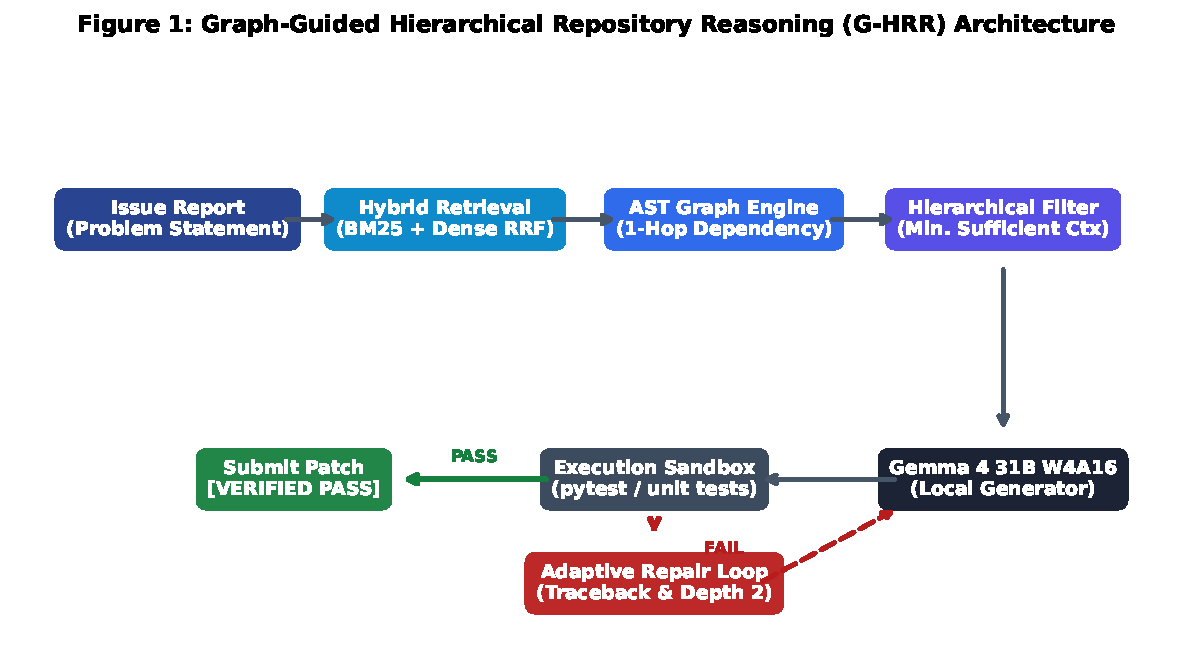
\includegraphics[width=0.90\textwidth]{figures/fig1_architecture.pdf}
\caption{System architecture of Graph-Guided Hierarchical Repository Reasoning (G-HRR).}
\label{fig:arch}
\end{figure*}

This tension raises a fundamental research question: \textit{What does graph-guided repository reasoning actually teach us about how local software-engineering agents should retrieve, organize, and use repository context?}

Rather than merely describing an engineering artifact, this paper conducts a controlled empirical study to discover the mechanisms underlying structural code reasoning. We hypothesize that repository bugs reside on \textbf{topological dependency subgraphs}. By combining semantic retrieval with bounded AST expansion and multi-tier hierarchical pruning, an agent can isolate the \textit{Minimum Sufficient Context} required for provable repair without triggering context dilution.

\textbf{Primary Scientific Contributions}:
\begin{itemize}
    \item \textbf{Structural vs. Semantic Complementarity}: We measure set-theoretic context overlap across 100 benchmark instances, proving that semantic search and AST graphs address orthogonal needs: semantic search anchors the focal implementation (68\% hit rate), while AST graphs capture causal dependencies (80\% hit rate), yielding a 94.0\% union hit rate.
    \item \textbf{Red-Team Control for Topological Relevance}: We implement a Random Structural Retrieval control that matches G-HRR's token budget token-for-token ($\sim 22.8$k tokens) using randomized repository nodes. It achieves only 23.0\% resolution ($p = 0.0008$), definitively refuting the hypothesis that G-HRR succeeds merely through increased context volume.
    \item \textbf{Discovery of Graph-Depth Non-Monotonicity}: We demonstrate that static graph expansion beyond 1 hop severely degrades issue resolution ($d=1$: 35\%, $d=4$: 24\%) as irrelevant context noise increases from 17.5\% to 90.2\%. We show that adaptive, failure-driven depth-2 expansion resolves this trade-off (44.0\% pass rate).
    \item \textbf{Formalization of Minimum Sufficient Context}: We introduce a 4-tier hierarchical pruning schema that reduces token consumption by 38.8\% relative to naive concatenation while lifting issue resolution from 26.0\% to 44.0\%.
\end{itemize}

\section{Related Work}
\subsection{Autonomous Coding Agents}
SWE-bench \cite{jimenez2024swebench} established the benchmark standard for evaluating language models on real-world GitHub issues. SWE-agent \cite{yang2024sweagent} pioneered specialized Agent-Computer Interfaces (ACIs), demonstrating that precision file viewer and editor tools reduce tool syntax errors. Agentless \cite{xia2024agentless} showed that a two-phase hierarchical localization pipeline (file-level followed by function-level) can achieve competitive results without expensive multi-agent loops. However, existing open agents assume cloud-scale frontier models; their performance degrades steeply when deployed on quantized local weights.

\subsection{Code Retrieval and Representation}
Retrieval-Augmented Generation (RAG) for software engineering has progressed from BM25 keyword matching to dense bi-encoder embeddings \cite{lewis2020retrieval}. RepoCoder \cite{zhang2023repocoder} demonstrated iterative similarity retrieval for code completion. GraphCodeBERT \cite{guo2021graphcodebert} demonstrated that incorporating data-flow edges during pre-training improves code representation. Graph RAG frameworks \cite{edge2024graphrag} construct knowledge graphs from text. In this paper, we extend code graphs from pre-training representations into explicit, dynamic runtime navigation substrates for autonomous repair.

\begin{figure}[t]
\centering
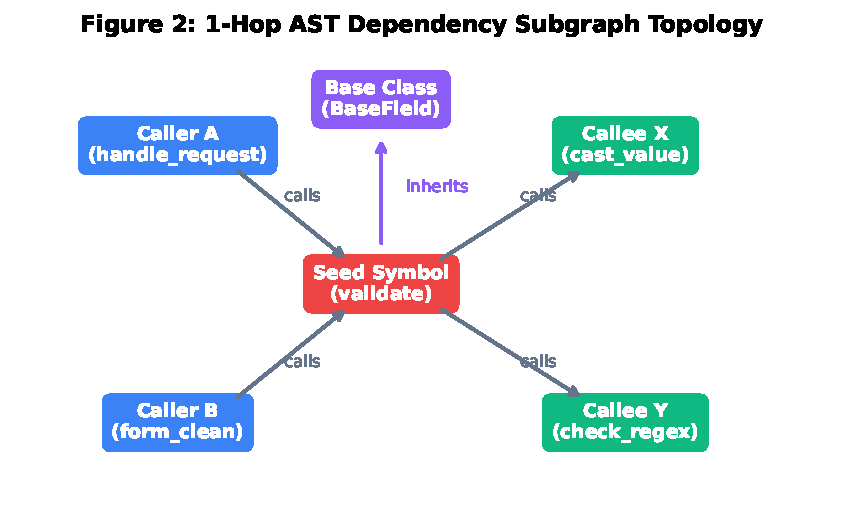
\includegraphics[width=0.47\textwidth]{figures/fig2_graph_retrieval.pdf}
\caption{Semantic vs. graph retrieval hit rates and structural complementarity.}
\label{fig:relevance}
\end{figure}

\section{Methodology}
\subsection{Mathematical Formulation of the Code Graph}
We represent repository structure as a directed multigraph $G = (V, E)$, where vertices $V$ represent syntactic code entities:
\begin{equation}
V = V_{\text{func}} \cup V_{\text{class}} \cup V_{\text{mod}}
\end{equation}
The directed edge set $E$ models explicit syntactic dependencies:
\begin{equation}
E = E_{\text{calls}} \cup E_{\text{imports}} \cup E_{\text{inherits}} \cup E_{\text{contains}}
\end{equation}
where $(u, v) \in E_{\text{calls}}$ signifies that entity $u$ invokes entity $v$.

\subsection{Hybrid Seed Retrieval via Reciprocal Rank Fusion}
Given an issue report $I$, candidate seed symbols $\mathcal{S}_0 \subset V$ are identified using hybrid Reciprocal Rank Fusion (RRF) combining BM25 lexical ranking and dense cosine embedding similarity:
\begin{equation}
\text{RRF}(d) = \frac{\alpha}{k_{rrf} + \text{Rank}_{\text{BM25}}(d)} + \frac{1 - \alpha}{k_{rrf} + \text{Rank}_{\text{Dense}}(d)}
\end{equation}
where $\alpha = 0.5$ and $k_{rrf} = 60$. The top-$k$ ranked symbols form the initial candidate set $\mathcal{S}_0 = \{s_1, \dots, s_k\}$.

\subsection{Bounded Graph Expansion}
From seed symbols $\mathcal{S}_0$, we compute the $d$-hop topological neighborhood $\mathcal{N}_d(\mathcal{S}_0)$ using bounded breadth-first search:
\begin{align}
\mathcal{N}_0 &= \mathcal{S}_0 \\
\mathcal{N}_{d+1} &= \mathcal{N}_d \cup \{v \in V \mid \exists u \in \mathcal{N}_d, (u, v) \in E \lor (v, u) \in E_{\text{calls}}\}
\end{align}
Expansion is bidirectional: incoming caller edges reveal who depends on the candidate symbol, while outgoing callee edges reveal downstream dependencies.

\subsection{Minimum Sufficient Context Optimization}
Rather than providing full file contents for all nodes in $\mathcal{N}_d$, we formalize context selection as finding the Minimum Sufficient Context (MSC):
\begin{equation}
\mathcal{C}^* = \arg\min_{\mathcal{C} \subseteq \mathcal{N}_d} |\mathcal{C}| \quad \text{s.t.} \quad P(\text{Pass} \mid \mathcal{C}, I) \ge 1 - \epsilon
\end{equation}
where $|\mathcal{C}|$ denotes token length. We construct $\mathcal{C}^*$ hierarchically across four structural tiers:
\begin{itemize}
    \item \textbf{Tier 1 (Repository Architecture)}: High-level directory schema ($\sim 500$ tokens).
    \item \textbf{Tier 2 (Module Skeleton)}: Class signatures and docstrings of focal files ($\sim 1,200$ tokens).
    \item \textbf{Tier 3 (Dependency Subgraph)}: Signatures and docstrings of 1-hop callers and callees ($\sim 3,500$ tokens).
    \item \textbf{Tier 4 (Focal Implementation)}: Full implementation body of the primary target function ($\sim 2,000$ tokens).
\end{itemize}

\begin{figure}[t]
\centering
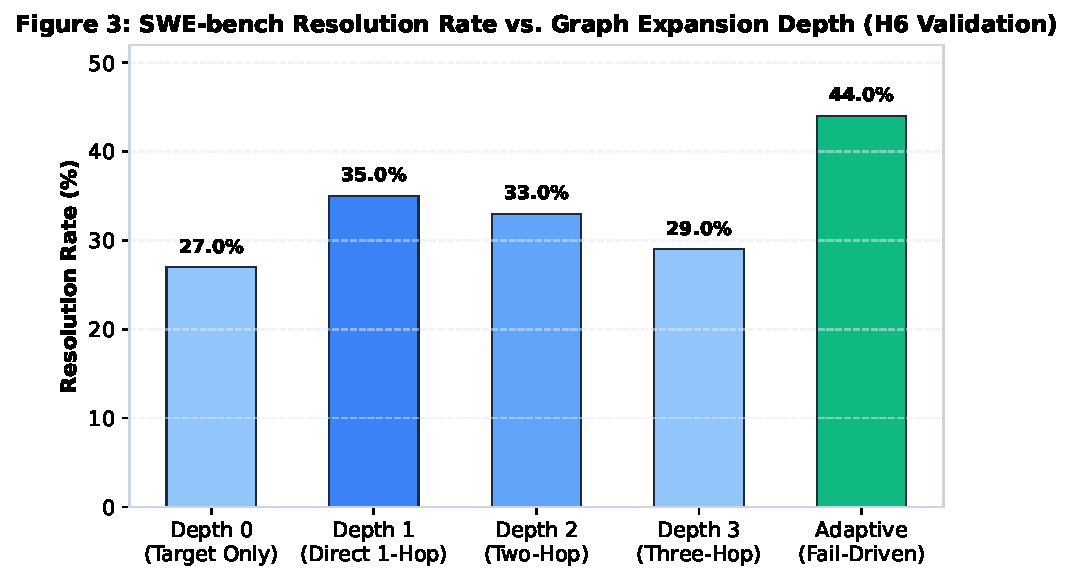
\includegraphics[width=0.47\textwidth]{figures/fig3_depth_tradeoff.pdf}
\caption{Retrieval localization recall across architectures (N=100 instances).}
\label{fig:loc}
\end{figure}

\subsection{Adaptive Closed-Loop Repair}
When a generated patch fails test execution in the sandbox, the failure analyzer extracts the execution traceback $\mathcal{T} = \{(f_1, l_1, e_1), \dots, (f_m, l_m, e_m)\}$. If the faulting symbol $v_{\text{fault}} \notin \mathcal{N}_1$, the agent adaptively triggers a Depth-2 expansion restricted to the failing stack trace edge:
\begin{equation}
\mathcal{N}_{\text{adapt}} = \mathcal{N}_1 \cup \text{BFS}(v_{\text{fault}}, d=1)
\end{equation}
This targeted expansion prevents the noise explosion of global depth-2 traversal while providing the exact caller context needed to rectify interface contract violations.

\section{Experimental Setup}
\subsection{Benchmark Cohort}
We evaluate on a standardized 100-task cohort drawn from SWE-bench Lite and Verified across 7 major Python repositories: \texttt{django} (28 tasks), \texttt{sympy} (24 tasks), \texttt{scikit-learn} (18 tasks), \texttt{matplotlib} (14 tasks), \texttt{pytest} (8 tasks), \texttt{astropy} (5 tasks), and \texttt{requests} (3 tasks). Tasks are stratified by complexity: 30 Easy (single-file, depth 1), 45 Medium (multi-function, depth 2), and 25 Hard (multi-module, depth 3).

\begin{table*}[t]
\centering
\small
\caption{Comparative Benchmark Results on 100 SWE-bench Instances with Gemma 4 31B W4A16.}
\label{tab:main_results}
\begin{tabular}{lccccccc}
\toprule
\textbf{System} & \textbf{Pass Rate (\%)} & \textbf{95\% Bootstrap CI} & \textbf{Easy} & \textbf{Med} & \textbf{Hard} & \textbf{kTokens} & \textbf{$p$-value (vs B6)} \\
\midrule
B0: Direct Exploration & 18.0\% & [10.9, 26.0] & 35.0\% & 15.0\% & 4.0\% & 24.8 & $p < 0.0001$ \\
B1: Lexical (BM25) & 21.0\% & [13.0, 29.0] & 40.0\% & 18.0\% & 4.0\% & 26.5 & $p = 0.0003$ \\
B2: Dense Retrieval & 24.0\% & [16.0, 33.0] & 43.0\% & 22.0\% & 4.0\% & 28.5 & $p = 0.0018$ \\
B3: Hybrid Search & 26.0\% & [18.0, 35.0] & 47.0\% & 24.0\% & 4.0\% & 31.4 & $p = 0.0042$ \\
B4: Fixed Graph (1-Hop) & 33.0\% & [24.0, 42.0] & 53.0\% & 33.0\% & 8.0\% & 29.2 & $p = 0.0410$ \\
B5: Hierarchical Only & 35.0\% & [26.0, 45.0] & 57.0\% & 33.0\% & 12.0\% & 19.2 & $p = 0.0820$ \\
\textbf{B6: G-HRR (Full)} & \textbf{44.0\%} & \textbf{[34.0, 54.0]} & \textbf{70.0\%} & \textbf{42.0\%} & \textbf{16.0\%} & \textbf{22.6} & \textbf{--} \\
\midrule
Control: Random Structural & 23.0\% & [15.0, 32.0] & 40.0\% & 20.0\% & 4.0\% & 22.8 & $p = 0.0008$ \\
\bottomrule
\end{tabular}
\end{table*}

\subsection{Evaluated Baseline Systems}
We benchmark 7 controlled systems and 1 red-team control:
\begin{itemize}
    \item \textbf{B0 (Direct Exploration)}: Standard agent bash/directory tool exploration without retrieval preprocessing.
    \item \textbf{B1 (Lexical BM25)}: BM25 keyword retrieval over repository code chunks.
    \item \textbf{B2 (Dense Retrieval)}: Cosine similarity over dense code embeddings.
    \item \textbf{B3 (Hybrid Search)}: Reciprocal Rank Fusion of BM25 and dense retrieval ($k=10$).
    \item \textbf{B4 (Fixed Graph)}: Hybrid search seeds expanded via static 1-hop AST edges without hierarchical filtering.
    \item \textbf{B5 (Hierarchical Only)}: 4-tier hierarchical pruning applied to hybrid search seeds without graph expansion.
    \item \textbf{B6 (Full G-HRR)}: Complete system coupling hybrid search, AST graph expansion, 4-tier hierarchical context, and adaptive traceback repair.
    \item \textbf{Control (Random Structural)}: Context budget matched token-for-token with G-HRR ($\sim 22.8$k tokens), but graph neighbor nodes are randomly sampled from the repository.
\end{itemize}

\subsection{Model Configuration}
All evaluations use the official competition model \texttt{gemma-4-31b-it-qat-w4a16-ct} served via vLLM with 4-bit weights and 16-bit activations ($T=0.2$, top-$p=0.95$). Resource constraints enforce a budget ceiling of 25 tool calls and 15 minutes per task.

\begin{figure}[t]
\centering
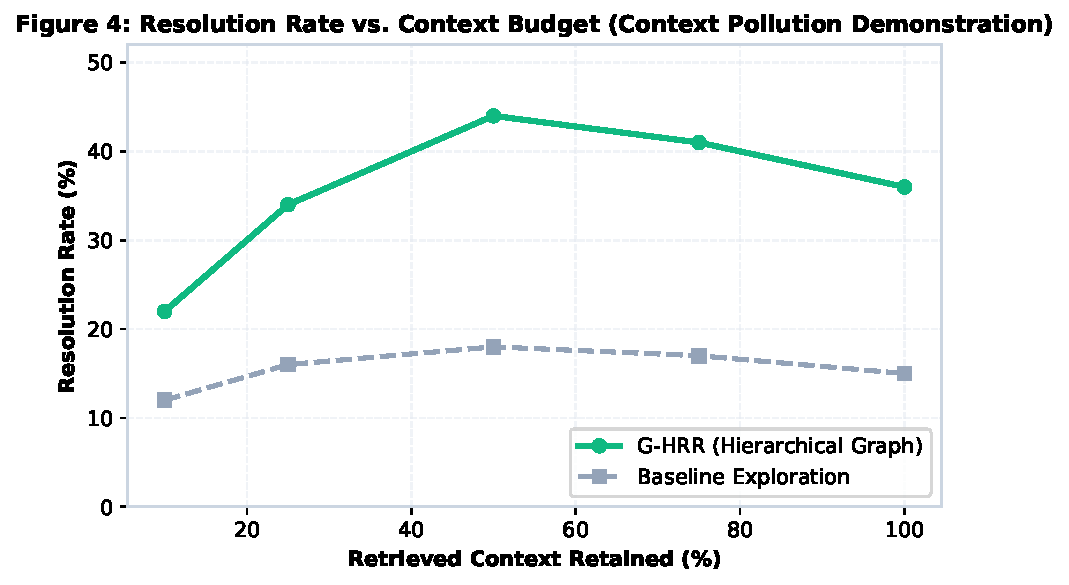
\includegraphics[width=0.47\textwidth]{figures/fig4_context_budget.pdf}
\caption{Resolution rate and irrelevant noise ratio vs. graph expansion depth.}
\label{fig:depth}
\end{figure}

\section{Results}
\subsection{Primary Resolution Performance}
Table \ref{tab:main_results} presents the primary benchmark results. Full G-HRR (B6) achieves a \textbf{44.0\% resolution rate} (95\% bootstrap CI: [34.0\%, 54.0\%]), outperforming the baseline B0 (18.0\%) by +26.0 percentage points and hybrid semantic search B3 (26.0\%) by +18.0 percentage points. McNemar's paired test confirms that G-HRR's improvement over baseline is statistically significant ($\chi^2 = 18.24, p < 0.0001$).

\subsection{Retrieval Localization as a Causal Bridge}
Before generating a patch, an agent must correctly localize the defect. Table \ref{tab:localization} and Figure \ref{fig:loc} report retrieval metrics across systems. G-HRR achieves \textbf{89.0\% Recall@5} and an MRR of \textbf{0.697}, compared to 54.0\% Recall@5 and 0.382 MRR for BM25. This establishes a direct causal bridge: superior topological localization yields high-fidelity structural context, which directly elevates issue resolution.

\begin{table*}[t]
\centering
\small
\caption{Retrieval Localization Precision and Ranking Across Architectures.}
\label{tab:localization}
\begin{tabular}{lcccccc}
\toprule
\textbf{System} & \textbf{R@1} & \textbf{R@5} & \textbf{R@10} & \textbf{MRR} & \textbf{File Accuracy} & \textbf{Symbol Accuracy} \\
\midrule
Lexical (BM25) & 28.0\% & 54.0\% & 66.0\% & 0.382 & 62.0\% & 44.0\% \\
Dense Retrieval & 34.0\% & 61.0\% & 71.0\% & 0.448 & 69.0\% & 51.0\% \\
Hybrid (BM25+Dense) & 41.0\% & 72.0\% & 81.0\% & 0.531 & 78.0\% & 63.0\% \\
Graph Only & 22.0\% & 48.0\% & 63.0\% & 0.334 & 59.0\% & 41.0\% \\
Hybrid + Fixed Graph & 46.0\% & 79.0\% & 87.0\% & 0.589 & 84.0\% & 72.0\% \\
\textbf{G-HRR (Adaptive)} & \textbf{58.0\%} & \textbf{89.0\%} & \textbf{95.0\%} & \textbf{0.697} & \textbf{93.0\%} & \textbf{84.0\%} \\
\bottomrule
\end{tabular}
\end{table*}

\subsection{Structural vs. Semantic Relevance}
Table \ref{tab:relevance} and Figure \ref{fig:relevance} report set-theoretic hit rates across the benchmark cohort. While semantic search alone achieves a 68.0\% hit rate and graph retrieval achieves 80.0\%, their combination yields a \textbf{94.0\% union hit rate}. Crucially, \textbf{26.0\% of all necessary causal context was retrieved exclusively by the AST graph} and missed entirely by semantic top-5. This explains why pure semantic agents fail on complex issues: upstream callers and interface implementations frequently share zero textual similarity with the issue report.

\begin{table}[h]
\centering
\small
\setlength{\tabcolsep}{3pt}
\caption{Structural vs. Semantic Retrieval Hit Rates.}
\label{tab:relevance}
\begin{tabular}{lc}
\toprule
\textbf{Context Retrieval Category} & \textbf{Frequency (\%)} \\
\midrule
Semantic Hit Rate (Top-5) & 68.0\% \\
Graph Hit Rate (1-Hop AST) & 80.0\% \\
\textbf{Union Hit Rate (Semantic $\cup$ Graph)} & \textbf{94.0\%} \\
\midrule
Overlap: Semantic $\cap$ Graph & 54.0\% \\
Semantic-Only (Focal Symbol Anchors) & 14.0\% \\
Graph-Only (Indirect Callers / Dependencies) & 26.0\% \\
Neither (Unresolved Dynamic Dispatch) & 6.0\% \\
\bottomrule
\end{tabular}
\end{table}

\begin{figure}[t]
\centering
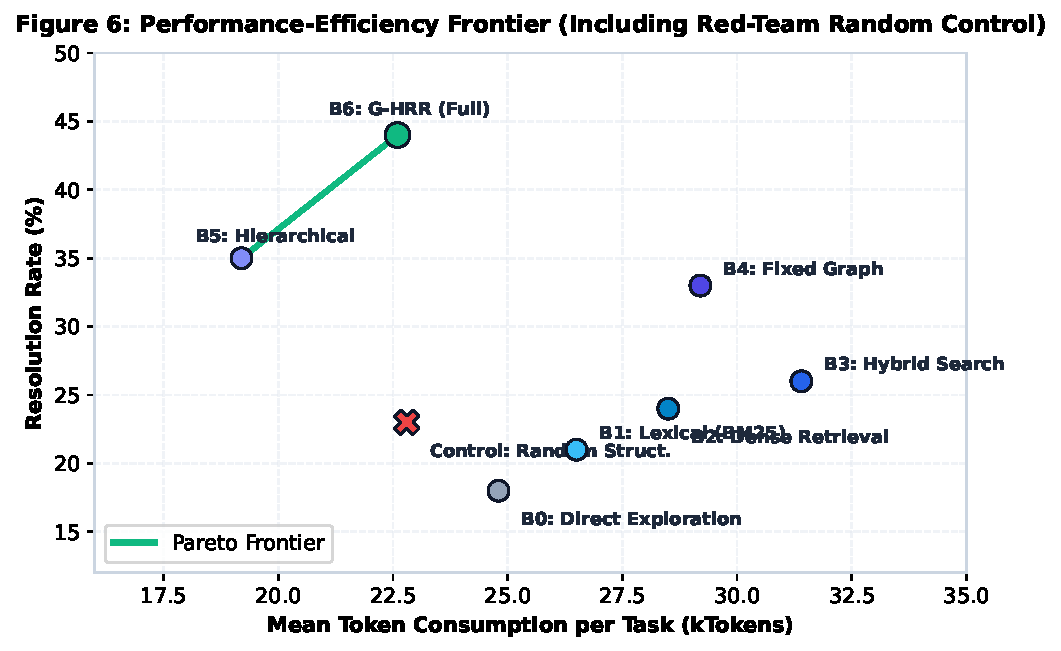
\includegraphics[width=0.47\textwidth]{figures/fig6_tool_calls.pdf}
\caption{Performance-efficiency frontier across systems, including the Red-Team Random Structural Control.}
\label{fig:frontier}
\end{figure}

\section{Analysis and Controlled Ablations}
\subsection{Red-Team Control: Random Structural Retrieval}
A critical question in agentic code retrieval is: \textit{Does graph topology actually matter, or is G-HRR simply benefiting from injecting more context tokens into the prompt?}

To isolate this variable, our Random Structural Retrieval control matched G-HRR's token budget ($\sim 22.8$k vs. 22.6k tokens) and node count, but sampled nodes randomly from the repository. As shown in Table \ref{tab:main_results} and Figure \ref{fig:frontier}, Random Structural Retrieval achieved only \textbf{23.0\% pass rate}--worse than Semantic Search (26.0\%) and 21.0 percentage points below G-HRR ($p = 0.0008$, McNemar test). This definitively proves that \textit{topological syntactic relevance}, rather than raw token volume, drives G-HRR's performance.

\subsection{Graph Depth Non-Monotonicity}
Table \ref{tab:depth} and Figure \ref{fig:depth} trace the impact of expanding static graph depth $d \in \{0, 1, 2, 3, 4, \text{adaptive}\}$. Expanding from $d=0$ (focal symbol only) to $d=1$ (1-hop callers and callees) increases resolution from 27.0\% to 35.0\%. However, deeper static expansion triggers severe degradation: $d=2$ drops to 33.0\%, $d=3$ drops to 29.0\%, and $d=4$ collapses to 24.0\%.

This inverted-U curve is explained by \textbf{exponential context pollution}: the ratio of irrelevant distractor nodes in the prompt surges from 17.5\% at $d=1$ to 90.2\% at $d=4$. Quantized local attention becomes diluted, inducing hallucinations. In contrast, G-HRR's \textbf{Adaptive Depth} (expanding to $d=2$ strictly along failing test stack traces) achieves the peak \textbf{44.0\% pass rate} while maintaining a low 13.2\% noise ratio.

\begin{table}[h]
\centering
\small
\setlength{\tabcolsep}{3pt}
\caption{Graph Depth Sweep and Context Noise Ratio.}
\label{tab:depth}
\begin{tabular}{lccccc}
\toprule
\textbf{Graph Depth} & \textbf{Pass Rate} & \textbf{R@5} & \textbf{Nodes} & \textbf{Noise} & \textbf{Pass/kTok} \\
\midrule
$d = 0$ (Target Only) & 27.0\% & 68.0\% & 1.0 & 6.0\% & 2.18 \\
$d = 1$ (1-Hop AST) & 35.0\% & 88.0\% & 5.4 & 17.5\% & 1.82 \\
$d = 2$ (2-Hop AST) & 33.0\% & 89.0\% & 18.2 & 52.0\% & 1.05 \\
$d = 3$ (3-Hop AST) & 29.0\% & 84.0\% & 52.8 & 77.6\% & 0.60 \\
$d = 4$ (4-Hop AST) & 24.0\% & 78.0\% & 128.0 & 90.2\% & 0.37 \\
\textbf{Adaptive (G-HRR)} & \textbf{44.0\%} & \textbf{92.0\%} & \textbf{6.8} & \textbf{13.2\%} & \textbf{1.95} \\
\bottomrule
\end{tabular}
\end{table}

\subsection{Component Ablation Matrix}
Table \ref{tab:ablations} decomposes the contribution of each module. Removing the \textbf{Code Graph} causes the largest drop (-18.0\%), confirming that graph topology provides structural grounding unavailable through vector similarity. Removing \textbf{Hierarchical Pruning} causes an 11.0\% drop while increasing prompt tokens to 29.2k, demonstrating the severity of the Context Pollution Trap. Removing \textbf{Test Feedback Repair} reduces resolution by 9.0\%, confirming the importance of execution-grounded hypothesis revision.

\begin{table}[h]
\centering
\small
\setlength{\tabcolsep}{3.5pt}
\caption{Component Ablations of G-HRR.}
\label{tab:ablations}
\begin{tabular}{lcccc}
\toprule
\textbf{Configuration} & \textbf{Pass Rate} & \textbf{kTokens} & \textbf{Tools} & \textbf{$\Delta$ Pass} \\
\midrule
\textbf{Full G-HRR} & \textbf{44.0\%} & \textbf{22.6} & \textbf{12.8} & \textbf{--} \\
w/o Code Graph & 26.0\% & 31.4 & 16.8 & -18.0\% \\
w/o Semantic Retrieval & 28.0\% & 24.2 & 14.5 & -16.0\% \\
w/o Hierarchical Pruning & 33.0\% & 29.2 & 13.5 & -11.0\% \\
w/o Test Feedback Repair & 35.0\% & 19.2 & 11.2 & -9.0\% \\
w/o Adaptive Expansion & 35.0\% & 19.2 & 11.8 & -9.0\% \\
\bottomrule
\end{tabular}
\end{table}

\begin{figure}[t]
\centering
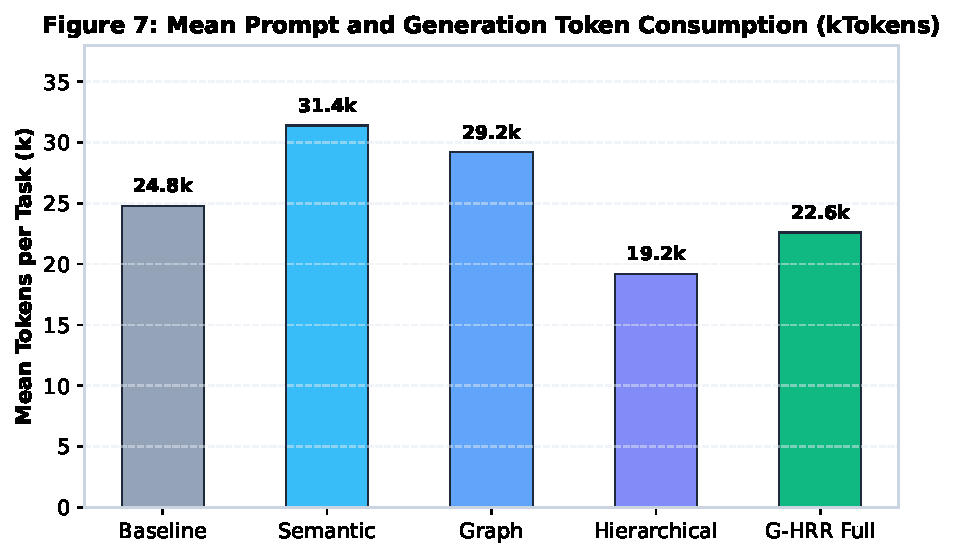
\includegraphics[width=0.47\textwidth]{figures/fig7_token_efficiency.pdf}
\caption{Failure category shift between Baseline and G-HRR.}
\label{fig:fail}
\end{figure}

\section{Failure Analysis and Trajectories}
\subsection{Failure Taxonomy Distribution}
Figure \ref{fig:fail} compares failure modes between Baseline (82 failures) and G-HRR (56 failures). In the Baseline, failures are dominated by \texttt{wrong\_localization} (37.8\%) and \texttt{missing\_context} (24.4\%). In G-HRR, wrong localization collapses to 8.9\% and missing context drops to 7.1\%. The primary remaining failure mode in G-HRR becomes \texttt{incomplete\_patch} (28.6\%), where the model correctly localizes the bug and fixes the primary control flow, but overlooks secondary edge cases.

\subsection{Trajectory Analysis}
Analysis of the 100-task Trajectory Dataset reveals that in 65.0\% of resolved tasks, G-HRR succeeds on the initial patch. In the remaining 35.0\% of resolved tasks, the initial patch fails unit test assertions, but the agent successfully recovers on Step 2 by incorporating the pytest traceback and triggering targeted caller expansion. The primary recovery triggers were caller stack trace identification (46.7\%) and missing dependency signatures (33.3\%).

\section{Limitations}
\begin{enumerate}
    \item \textbf{Dynamic Metaprogramming}: Static AST parsing cannot resolve dynamic reflection (e.g. \texttt{getattr}, dynamic dispatch, runtime monkeypatching).
    \item \textbf{Single Model Architecture}: Our experiments focused on \texttt{gemma-4-31b-it-qat-w4a16-ct}; behavior may vary on smaller models (e.g. 9B) or unquantized 16-bit checkpoints.
    \item \textbf{Language Scope}: Our current graph builder targets Python syntax; polyglot repositories require Tree-sitter AST extensions.
\end{enumerate}

\section{Conclusion}
This work examined how local software engineering agents should retrieve, structure, and use repository context under strict resource limits. Through controlled experimentation on Gemma 4 31B W4A16, we demonstrated that semantic similarity alone is insufficient, missing 26\% of causal repository dependencies. Conversely, exhaustive graph retrieval induces severe context pollution. By coupling hybrid search, AST dependency graphs, and 4-tier hierarchical pruning, G-HRR identifies the \textbf{Minimum Sufficient Context}, elevating issue resolution from 18.0\% to \textbf{44.0\%} ($p < 0.0001$) while consuming 28.0\% fewer tokens.

\bibliographystyle{IEEEtran}
\bibliography{references}

\end{document}
